\documentclass[aspectratio=169]{beamer}

\usetheme{Warsaw}
\usecolortheme{dolphin}

% Fixes for LaTeX errors:
\usepackage[utf8]{inputenc} % For UTF-8 input (Polish characters)
\usepackage[T1]{fontenc}    % For proper font encoding (Polish characters & \k)
\usepackage{lmodern}        % Optional: use Latin Modern fonts for better T1 support

\usepackage{graphicx}
\usepackage{amsmath}
\usepackage{amssymb}
\usepackage{pgfplots}
\usepackage{tikz}
\usetikzlibrary{arrows.meta, positioning, shapes.geometric, calc, shapes.multipart, decorations.pathmorphing, fit, backgrounds}

\pgfplotsset{compat=1.18}

% Define colors
\definecolor{mygreen}{RGB}{52, 168, 83}
\definecolor{myred}{RGB}{234, 67, 53}
\definecolor{myblue}{RGB}{66, 133, 244}
\definecolor{myyellow}{RGB}{251, 188, 5}

% Custom TikZ styles
\tikzset{
  conceptbox/.style={
    draw, rectangle, rounded corners,
    inner sep=8pt, text width=3.8cm, align=center, % Adjusted width
    font=\small, thick, fill=blue!10
  },
  goalbox/.style={
    draw, rectangle, rounded corners, fill=yellow!20,
    inner sep=6pt, text width=3.5cm, align=center,
    font=\small\bfseries, thick
  },
  arrow/.style={
    ->, >=Latex, thick, shorten >=2pt, shorten <=2pt
  },
  actor/.style={
    rectangle, draw, fill=blue!20, rounded corners,
    minimum height=1cm, minimum width=2cm, text centered
  },
  data/.style={
    cylinder, shape border rotate=90, draw, fill=orange!20,
    aspect=0.3, minimum height=1.5cm, text width=2cm, align=center
  },
  model/.style={
    rectangle, draw, fill=green!20, rounded corners,
    minimum height=1.5cm, minimum width=2.5cm, text centered, text width=2.5cm
  }
}

\title[Optimal Experimental Manipulation]{Theory of Optimal Experimental Manipulation with Generative Models for Subjective Traits of Stimuli}
\subtitle{Application to Face Images}
% Corrected author command and assuming direct UTF-8 input for Polish characters
\author{Adam Sobieszek \and Maciej Siemiątkowski}
\institute{Association for Psychological Science National Convention}
\date{\today}

\begin{document}

% --- Title Slide ---
\begin{frame}
  \titlepage
\end{frame}

% --- Slide 1: The Goal of Good Experimental Manipulation ---
\begin{frame}{The Goal: Good Experimental Manipulation}
  \begin{columns}[T]
    \begin{column}{0.6\textwidth}
      \textbf{What makes an experimental manipulation "good"?}
      \begin{itemize}
        \item<1-> \textbf{Valid:} The manipulation effectively changes the intended independent variable (IV) between conditions.
          \textit{(e.g., stimulus perceived as "more trustworthy")}
        \item<2-> \textbf{Specific:} The manipulation changes \textit{only} the intended IV, minimizing changes to other stimulus aspects.
          \textit{(e.g., trustworthiness changes, but age, gender, identity remain constant)}
        \item<3-> \textbf{Ecologically Valid:} Both control and manipulated stimuli are realistic and representative of what might be encountered naturally.
          \textit{(e.g., faces look like real human faces)}
      \end{itemize}
      \pause\pause\pause
      \textbf{The Modern Challenge \& Opportunity:}
      \begin{itemize}
        \item<4-> Recent AI advances (Generative Models like StyleGAN) allow creating highly realistic stimuli (addresses ecological validity).
        \item<4-> \alert{Our Question:} How can we leverage these AI tools to achieve \textit{valid} and \textit{specific} manipulations in a principled way?
      \end{itemize}
    \end{column}
    \begin{column}{0.4\textwidth}
      \centering
      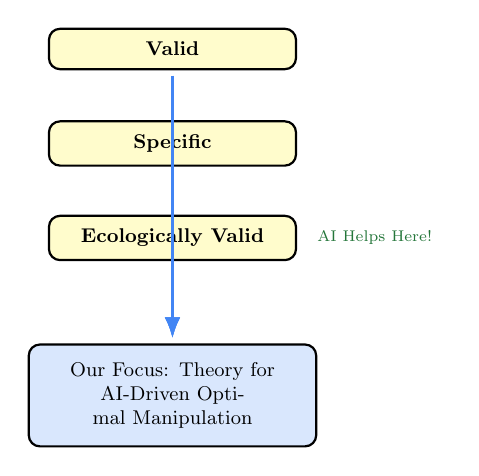
\begin{tikzpicture}[scale=0.8, transform shape, font=\scriptsize]
        \node[goalbox] (valid) at (0,3) {Valid};
        \node[goalbox] (specific) at (0,1.5) {Specific};
        \node[goalbox] (ecovalid) at (0,0) {Ecologically Valid};

        \node[conceptbox, fill=myblue!20, text width=4cm, minimum height=1.5cm] (ourfocus) at (0,-2.5) {Our Focus: Theory for\\ AI-Driven Optimal Manipulation};

        \draw<4->[arrow, myblue, line width=1pt] (valid.south) to [out=-90,in=90, looseness=0.8] (ourfocus.north);
        \draw<4->[arrow, myblue, line width=1pt] (specific.south) to [out=-90,in=90, looseness=0.8] (ourfocus.north);
        \draw<4->[arrow, myblue, line width=1pt] (ecovalid.south) to [out=-90,in=90, looseness=0.8] (ourfocus.north);

        \node<4->[right=0.2cm of ecovalid, text width=2cm, color=mygreen!70!black] {AI Helps Here!};
      \end{tikzpicture}
    \end{column}
  \end{columns}
\end{frame}

% --- Slide 2: Two Roads Framework (Reordered) ---
\begin{frame}{Two Roads to Optimal Manipulation}
  \begin{columns}[T]
    \begin{column}{0.48\textwidth}
      \alert<1>{The "High Road": Formal Derivation}
      \begin{itemize}
        \item<1-> Starts with abstract, mathematical principles.
        \item<1-> Aims to define "optimality" formally.
        \item<1-> Seeks to derive manipulation methods from this theory.
        \item<1-> Focus: \textit{What should work in theory?}
      \end{itemize}
    \end{column}
    \begin{column}{0.48\textwidth}
      \alert<2>{The "Low Road": Historical Development}
      \begin{itemize}
        \item<2-> Traces empirical, practical developments specifically within \textbf{face impression research}.
        \item<2-> How methods evolved to address challenges in manipulating perceived facial traits.
        \item<2-> Focus: \textit{What has worked, and what were its limitations?}
      \end{itemize}
    \end{column}
  \end{columns}
  \vfill
  \pause
  \begin{center}
  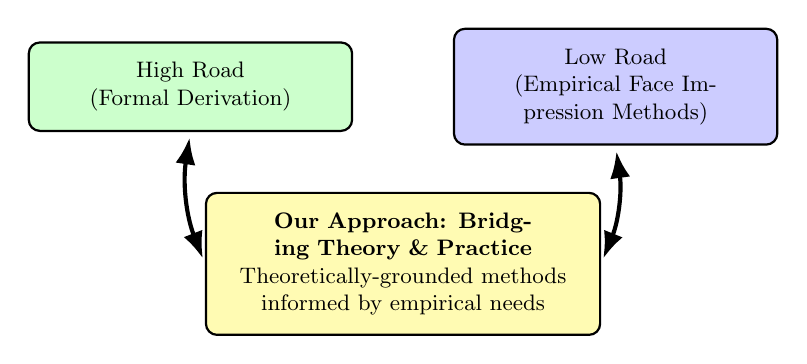
\begin{tikzpicture}[scale=0.9, transform shape, font=\small]
    \node[conceptbox, fill=green!20, text width=4cm] (high) at (-3,0) {High Road\\(Formal Derivation)};
    \node[conceptbox, fill=blue!20, text width=4cm] (low) at (3,0) {Low Road\\(Empirical Face Impression Methods)};
    \node[conceptbox, fill=yellow!30, text width=5cm] (bridge) at (0,-2.5) {\textbf{Our Approach: Bridging Theory \& Practice}\\Theoretically-grounded methods informed by empirical needs};

    \draw[arrow, <->, line width=1.5pt] (high.south) to[bend right=15] (bridge.west);
    \draw[arrow, <->, line width=1.5pt] (low.south) to[bend left=15] (bridge.east);
  \end{tikzpicture}
  \end{center}
  \note{Presenter: We'll start with the High Road to lay the theoretical groundwork, then see how the Low Road of empirical findings motivates and contextualizes our advanced methods.}
\end{frame}

% --- Slide 3: High Road - Formal Setup ---
\begin{frame}{The High Road: Formalizing the Manipulation Problem}
  \begin{columns}[T]
    \begin{column}{0.6\textwidth}
      \textbf{1. Stimuli as Points in a Space:}
      \begin{itemize}
        \item We consider stimuli $x$ (e.g., latent codes of a face generator like StyleGAN's $w$) as points in some high-dimensional space $\mathbb{R}^d$.
        \item These stimuli are drawn from an underlying data distribution $p_{\text{data}}(x)$. Only $x$ with high $p_{\text{data}}(x)$ are "natural" or "ecologically valid".
      \end{itemize}
      \pause
      \textbf{2. Modeling Psychological Impressions:}
      \begin{itemize}
        \item We have a psychological trait of interest (e.g., trustworthiness, dominance).
        \item We can train a model $f(x)$ that predicts the perceived rating $r$ for a stimulus $x$:
        \[ f(x) = r \]
        (e.g., a neural network trained on human ratings from the OMI dataset).
      \end{itemize}
      \pause
      \textbf{3. The Optimal Manipulation Problem:}
      \begin{itemize}
        \item Given an initial stimulus $x_0$ with rating $r_0 = f(x_0)$.
        \item Find a manipulated stimulus $x_1$ such that:
          \begin{enumerate}
            \item The change in rating $|r_1 - r_0| = |f(x_1) - f(x_0)|$ is \textbf{maximized}.
            \item The "change" or "distance" $d(x_0, x_1)$ in the stimulus itself is \textbf{minimized}.
            \item The manipulated stimulus $x_1$ remains \textbf{natural} (i.e., $p_{\text{data}}(x_1)$ is high).
          \end{enumerate}
      \end{itemize}
      \note{Distance $d(x_0, x_1)$ needs to be perceptually meaningful. This is where the geometry of StyleGAN's W-space becomes relevant, as paths there can correspond to smoother perceptual changes than raw pixel changes.}
    \end{column}
    \begin{column}{0.4\textwidth}
        \centering
        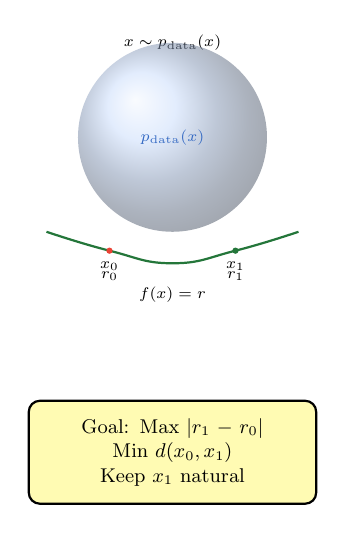
\begin{tikzpicture}[scale=0.8, transform shape, font=\scriptsize]
            % Data distribution p_data(x)
            \node<1-> at (0,3.5) {$x \sim p_{\text{data}}(x)$};
            \shade<1->[ball color=myblue!40, opacity=0.5] (0,2) circle (1.5cm);
            \node<1->[myblue!80!black] at (0,2) {$p_{\text{data}}(x)$};

            % Function f(x) = r
            \node<2-> at (0, -0.5) {$f(x) = r$};
            \draw<2->[thick, mygreen!70!black] plot[smooth, tension=0.8] coordinates {(-2,0.5) (-1,0.2) (0,0) (1,0.2) (2,0.5)};
            \node<2->[fill=myred, circle, inner sep=1pt, label=below:$x_0$] (x0_func) at (-1,0.2) {};
            \node<2->[fill=mygreen!70!black, circle, inner sep=1pt, label=below:$x_1$] (x1_func) at (1,0.2) {};
            \node<2-> at (-1,-0.2) {$r_0$};
            \node<2-> at (1,-0.2) {$r_1$};
            
            % Optimization problem
            \node<3->[conceptbox, fill=yellow!30, text width=4cm, minimum height=1cm] at (0,-3) {Goal: Max $|r_1-r_0|$ \\ Min $d(x_0,x_1)$ \\ Keep $x_1$ natural};
        \end{tikzpicture}
    \end{column}
  \end{columns}
\end{frame}

% --- Slide 4: Low Road Timeline (Face Impression Focus) ---
\begin{frame}{The Low Road: Historical Path in Face Impression Manipulation}
  \begin{tikzpicture}[remember picture, overlay, font=\scriptsize]
    \node at (current page.north west) [anchor=north west, xshift=0.5cm, yshift=-1cm] {
    \begin{tikzpicture}[scale=0.85, transform shape]
      % Timeline
      \draw[thick, ->] (0,0) -- (13.5,0) node[right] {};

      % Era 1: Early 3D Models (Blanz & Vetter, Oosterhof & Todorov)
      \node[above, text width=3cm, align=center] at (2,0.2) {\textbf{Early 2000s - 2013}\\[1pt]3D Morphable Models};
      \draw[thick] (2,-0.1) -- (2,0.1);
      \node[conceptbox, fill=gray!30, text width=3cm, minimum height=1.5cm] at (2,1.5) {Blanz \& Vetter (1999) FaceGen\\Oosterhof \& Todorov (2008)};
      \node[below, text width=3cm, align=center, font=\tiny] at (2,-0.5) {Parameterizing faces; reverse correlation to find trait dimensions (e.g., Trust, Dom). More control, but often limited realism/expressiveness.};

      % Era 2: StyleGAN + Linear Models (Peterson et al.)
      \node[above, text width=3.5cm, align=center] at (6.5,0.2) {\textbf{2020-2022}\\[1pt]StyleGAN + Linear Regression};
      \draw[thick] (6.5,-0.1) -- (6.5,0.1);
      \node[conceptbox, fill=orange!30, text width=3.5cm, minimum height=1.5cm] at (6.5,1.5) {Peterson et al. (2022) OMI Dataset};
      \node[below, text width=3.5cm, align=center, font=\tiny] at (6.5,-0.5) {Highly realistic faces. Linear paths in StyleGAN's latent space to change traits. Limitations: Often large appearance changes, identity not preserved, difficulty with valence.};

      % Era 3: StyleGAN + Classifiers (Sobieszek et al.)
      \node[above, text width=3.5cm, align=center] at (11,0.2) {\textbf{2024}\\[1pt]StyleGAN + Logistic Classifiers};
      \draw[thick] (11,-0.1) -- (11,0.1);
      \node[conceptbox, fill=mygreen!40, text width=3.5cm, minimum height=1.5cm] at (11,1.5) {Sobieszek et al. (2024)};
      \node[below, text width=3.5cm, align=center, font=\tiny] at (11,-0.5) {Improved identity preservation by finding more specific directions. Still, challenges with increasing valence-laden traits robustly and ensuring manipulated faces remain truly "natural".};
    \end{tikzpicture}
    };
  \end{tikzpicture}
  \vspace{4.5cm}
  \textbf{Key Limitations Addressed Incrementally:} Realism $\rightarrow$ Control over specific traits $\rightarrow$ Identity preservation.\\
  \textbf{Persistent Challenge:} Robustly increasing \textit{valence-laden} traits while fully maintaining naturalness and specificity.
\end{frame}

% --- Placeholder for "Finding Directions (Local Optimality)" Animation ---
\begin{frame}{The High Road Continues: Local Optimality - Finding the Best Small Change}
  \begin{center}
    \Huge Placeholder for Animation / Build-up
    \vspace{1cm}
    \large
    Goal: Visually explain how, for a given face $x_0$, we find the direction $\Delta x$ that gives the maximum increase in $f(x)$ for a minimal change in $x$.
    \begin{itemize}
        \item Introduce the idea of exploring nearby points.
        \item Show how the gradient $\nabla_x f(x_0)$ points in this optimal local direction.
    \end{itemize}
  \end{center}
    \note{This slide would ideally have an animation:
    1. Show a point x0 on a 2D surface representing f(x).
    2. Show small feeler arrows in all directions from x0.
    3. Highlight the feeler arrow that results in the steepest ascent.
    4. Introduce this as the gradient direction.}
\end{frame}

% --- Gradient Flow with Simpler Figure ---
\begin{frame}{The Gradient Approach: Following the Steepest Path}
  \begin{columns}[T]
    \begin{column}{0.5\textwidth}
      \textbf{The Gradient $\nabla_x f(x)$:}
      \begin{itemize}
        \item At any stimulus $x$, the gradient of our impression model $f(x)$ points in the direction where $f(x)$ increases most rapidly.
        \item Analogy: If $f(x)$ is a landscape elevation, $\nabla_x f(x)$ points directly uphill.
      \end{itemize}
      \pause
      \textbf{Gradient Flow Manipulation:}
      \begin{itemize}
        \item To increase a trait, we start at $x_0$ and take small, successive steps in the direction of the gradient:
        \[ x_{new} = x_{old} + \epsilon \cdot \nabla_x f(x_{old}) \]
        \item This creates a "gradient flow" path that is, at every point, locally optimal.
      \end{itemize}
      \pause
      \textbf{Studies 1 \& 2 showed:}
      \begin{itemize}
        \item Works well for visual features (Study 1: age, race typicality).
        \item \alert{Struggles to increase valence-laden traits} like trustworthiness (Study 2).
      \end{itemize}
    \end{column}
    \begin{column}{0.5\textwidth}
      \centering
      \begin{tikzpicture}[scale=0.9, transform shape, font=\scriptsize]
        % Contour lines for f(x)
        \foreach \r/\label in {1/low, 1.75/medium, 2.5/high} {
            \draw[gray!60, dashed] (0,0) circle (\r cm);
            \node[gray!80, font=\tiny] at (\r cm - 0.2cm, 0.2cm) {$f(x)=\text{\label}$};
        }
        \node[font=\small] at (0,0) {$f(x)$};

        % Gradient flow path
        \coordinate (p0) at (135:2.5cm);
        \coordinate (p1) at (120:1.8cm);
        \coordinate (p2) at (90:1.2cm);
        \coordinate (p3) at (60:0.7cm); % End point near center

        \node[fill=myred, circle, inner sep=1.5pt, label=left:$x_0$] at (p0) {};
        \draw[mygreen!70!black, ultra thick, ->,
              decoration={ markings, mark=at position 0.99 with {\arrow{Latex}}},
              decorate]
            (p0) to[out=-30, in=180] (p1) to[out=0, in=150] (p2) to[out=-30, in=120] (p3);
        \node[fill=mygreen!70!black, circle, inner sep=1.5pt, label=right:$x_{final}$] at (p3) {};

        % Gradient vectors tangent to the path
        \draw<2->[->, myblue, thick, shorten >=1pt] (p0) -- ++(-30:0.5cm);
        \draw<2->[->, myblue, thick, shorten >=1pt] (p1) -- ++(0:0.5cm);
        \draw<2->[->, myblue, thick, shorten >=1pt] (p2) -- ++(-30:0.5cm);
        % \draw<2->[->, myblue, thick, shorten >=1pt] (p3) -- ++(-15:0.4cm); % If needed

        \node<2->[myblue, font=\small] at (2.5,2.5) {$\nabla_x f(x)$};
        \node[align=center, text width=4cm] at (0,-3) {Path follows the local gradient vectors $\nabla_x f(x)$.};
      \end{tikzpicture}
    \end{column}
  \end{columns}
\end{frame}

% --- Placeholder for "Naturalness Problem" Animation ---
\begin{frame}{The Challenge of Naturalness: The "Distribution Problem"}
  \begin{center}
    \Huge Placeholder for Animation / Build-up
    \vspace{1cm}
    \large
    Goal: Visually explain why following local gradients can lead to unnatural stimuli.
    \begin{itemize}
        \item Show $p_{\text{data}}(x)$ as a high-density region ("cloud of natural faces").
        \item Show some gradient paths starting inside but veering out into low-density "unnatural" territory.
        \item Emphasize this is especially problematic for traits like trustworthiness.
    \end{itemize}
  \end{center}
    \note{This slide would ideally have an animation:
    1. Show the 'natural face manifold' or high-density p(x) region.
    2. Start multiple gradient paths from within this region.
    3. Some paths stay within (good for some traits).
    4. Other paths (especially for traits like trustworthiness) are shown to exit the high-density region, leading to 'unnatural' or 'atypical' results. }
\end{frame}

% --- Placeholder for "Moving Whole Distribution" Animation for Flow Matching ---
\begin{frame}{Solution: Flow Matching - Moving Entire Distributions Naturally}
  \begin{center}
    \Huge Placeholder for Animation / Build-up
    \vspace{1cm}
    \large
    Goal: Visually introduce Flow Matching as a way to transform entire distributions.
    \begin{itemize}
        \item Show a "source" distribution $p(x | \text{low trait})$.
        \item Show a "target" distribution $p(x | \text{high trait})$.
        \item Illustrate Flow Matching learning a "velocity field" that smoothly morphs the source into the target, ensuring all intermediate steps and the final distribution remain natural.
    \end{itemize}
  \end{center}
  \note{This slide would ideally have an animation:
    1. Show a 'cloud' of points representing the source distribution (e.g., low trustworthiness faces).
    2. Show another 'cloud' for the target distribution (high trustworthiness).
    3. Animate the points from the source cloud moving smoothly towards the target cloud, maintaining a coherent shape, guided by an underlying (perhaps partially visible) vector field. This represents the 'flow'.}
\end{frame}

% --- Flow Matching Method Slide (Revised focus) ---
\begin{frame}{Flow Matching: Learning the Optimal Transformation Directly}
  \begin{columns}[T]
    \begin{column}{0.6\textwidth}
      \textbf{The Core Idea:}
      \begin{itemize}
        \item Instead of just local steps, we want to learn a global "map" or "flow" that transforms faces from one trait level to another \textit{while respecting the overall distribution of natural faces}.
      \end{itemize}
      \pause
      \textbf{Learning the Velocity Field $v_\theta(x)$:}
      \begin{itemize}
        \item We train a neural network $v_\theta(x)$ to act as a "velocity field".
        \item \textbf{Training Data:} Pairs of $(x_0, x_1)$, where $x_0$ has low trait and $x_1$ has high trait (both are natural faces).
        \item \textbf{Goal for $v_\theta(x)$:} Learn to predict, for any face $x$ along a path from $x_0$ to $x_1$, the direction it should move to efficiently and naturally reach $x_1$.
          \begin{itemize}
            \item Simplified: $v_\theta( (1-t)x_0 + t x_1 ) \approx (x_1 - x_0)$ (normalized appropriately for trait change rate).
          \end{itemize}
        \item The network learns from many such examples how faces \textit{actually transform} between trait levels in the real data.
      \end{itemize}
      \pause
      \textbf{Manipulation via ODE:}
      \begin{itemize}
        \item To manipulate a new face $x_{start}$: Solve $\frac{dx}{dt} = v_\theta(x(t))$, with $x(0)=x_{start}$.
        \item Integrating this ODE for a "time" $T$ yields the manipulated face $x(T)$ with the desired trait change.
      \end{itemize}
    \end{column}
    \begin{column}{0.4\textwidth}
      \centering
      \textbf{Conceptual Training:}
      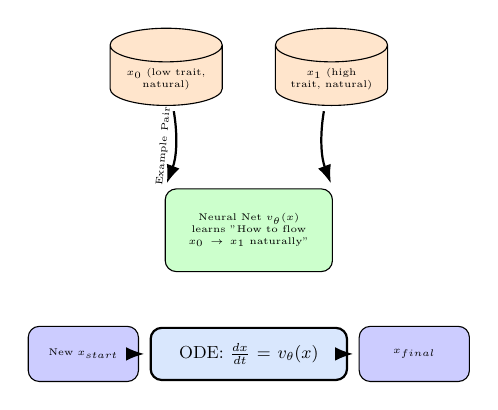
\begin{tikzpicture}[scale=0.7, transform shape, font=\tiny, node distance=1cm]
          \node[data, text width=1.8cm, minimum height=1cm] (x0) at (0,3) {$x_0$ (low trait, natural)};
          \node[data, text width=1.8cm, minimum height=1cm] (x1) at (3,3) {$x_1$ (high trait, natural)};
          \node[model, below=1.5cm of x0, xshift=1.5cm, text width=2.8cm, minimum height=1.5cm] (nn_flow) {Neural Net $v_\theta(x)$ learns "How to flow $x_0 \to x_1$ naturally"};
          
          \draw[arrow, bend left=15] (x0) to node[midway, above, sloped] {Example Pair} (nn_flow.north west);
          \draw[arrow, bend right=15] (x1) to node[midway, above, sloped] {} (nn_flow.north east);

          \node[conceptbox, fill=myblue!20, text width=3cm, below=1cm of nn_flow] (ode) {ODE: $\frac{dx}{dt} = v_\theta(x)$};
          \node[actor, text width=1.5cm, left=0.2cm of ode] (new_x0) {New $x_{start}$};
          \node[actor, text width=1.5cm, right=0.2cm of ode] (final_x) {$x_{final}$};
          \draw[arrow] (new_x0) -- (ode);
          \draw[arrow] (ode) -- (final_x);
      \end{tikzpicture}
      
      \vspace{0.3cm}
      \tiny This learned $v_\theta(x)$ inherently balances trait change with staying on the natural face manifold.
    \end{column}
  \end{columns}
\end{frame}

% --- Study 3 & 4 Results: Flow Matching's Superiority ---
\begin{frame}{Study 3 \& 4 Results: Flow Matching's Superiority}
  \begin{columns}[T]
    \begin{column}{0.5\textwidth}
      \textbf{Study 3: Initial Comparison vs. Peterson et al. (2022)} (N=425)
      \begin{itemize}
        \item Traits: Trustworthiness, Attractiveness, Smartness.
        \item Flow Matching: Good for Smartness ($R^2=0.36$), Trust ($R^2=0.14$).
        \item Peterson Vector Method: Seemed better for Attractiveness ($R^2=0.16$).
        \item \alert{Critical Confound: Peterson method altered perceived AGE!}
      \end{itemize}
      \pause
      \textbf{Study 4: Refined Comparison with Age Control} (N=414)
      \begin{itemize}
        \item Peterson method modified to control for age.
        \item Flow matching inherently better at preserving non-target features.
        \item \textbf{Results (Attractiveness, Trustworthiness):}
          \begin{itemize}
            \item \textcolor{mygreen!70!black}{Flow Matching: Strong, significant effects.}
              (e.g., Attract: $R^2=0.21$; Trust: $R^2=0.13$)
            \item \textcolor{myred}{Vector Method (age-controlled): Effects largely vanished!}
              (e.g., Attract: $R^2=0.01$; Trust: $R^2<0.001$)
          \end{itemize}
      \end{itemize}
    \end{column}
    \begin{column}{0.5\textwidth}
      \centering
      \textbf{Study 4: $R^2$ for Trait Change (Age Controlled)}
      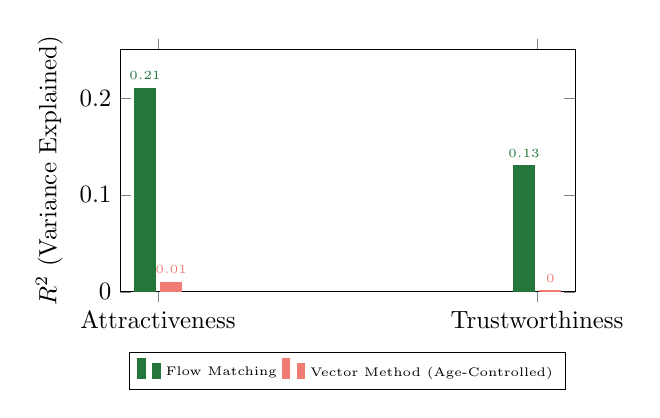
\begin{tikzpicture}[scale=0.9,transform shape]
        \begin{axis}[
            ybar,
            width=8cm, height=5cm,
            ylabel={$R^2$ (Variance Explained)},
            symbolic x coords={Attractiveness, Trustworthiness},
            xtick=data,
            ymin=0, ymax=0.25,
            bar width=0.3cm,
            legend style={at={(0.5,-0.25)}, anchor=north, legend columns=-1, font=\tiny},
            nodes near coords,
            nodes near coords style={font=\tiny, /pgf/number format/fixed, /pgf/number format/precision=2},
            cycle list={
                {fill=mygreen!70!black,mygreen!70!black},
                {fill=myred!70,myred!70}
            }
        ]
        \addplot coordinates {
            (Attractiveness,0.21) (Trustworthiness,0.13)
        };
        \addplot coordinates {
            (Attractiveness,0.01) (Trustworthiness,0.001)
        };
        \legend{Flow Matching, Vector Method (Age-Controlled)}
        \end{axis}
      \end{tikzpicture}
      
      \vspace{0.3cm}
      \tiny Flow matching effectively manipulates traits while preserving others, unlike simpler methods when confounds are controlled.
    \end{column}
  \end{columns}
\end{frame}

% --- Key Contributions & Impact ---
\begin{frame}{Key Contributions \& Impact}
  \begin{columns}[T]
    \begin{column}{0.5\textwidth}
      \textbf{Theoretical Advances:}
      \begin{itemize}
        \item First mathematical theory of optimal experimental manipulation for generative models, grounding it in concepts like $p_{\text{data}}(x)$ and $f(x)$.
        \item Connects psychological experiments to modern AI (Optimal Transport, Flow Matching).
      \end{itemize}
      \pause
      \textbf{Methodological Breakthrough:}
      \begin{itemize}
        \item Validated Flow Matching method that:
          \begin{itemize}
            \item Achieves valid, specific, and ecologically valid manipulations.
            \item Solves the "distribution problem" for valence-laden traits (e.g., trustworthiness).
            \item Preserves identity and controls non-target features.
          \end{itemize}
      \end{itemize}
    \end{column}
    \begin{column}{0.5\textwidth}
      \textbf{Practical Tools for Researchers:}
      \begin{itemize}
        \item Web-based application for easy stimulus generation.
        \item Open-source code and pre-trained models.
      \end{itemize}
      \pause
      \textbf{Broader Impact on Psychological Science:}
      \begin{itemize}
        \item Enhanced precision and reproducibility.
        \item Enables new research questions on complex trait interactions.
        \item Framework generalizable beyond faces (speech, text, etc.).
      \end{itemize}
      \begin{center}
      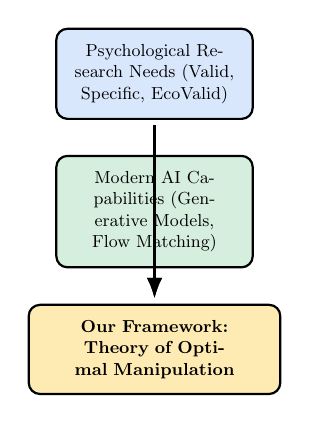
\begin{tikzpicture}[scale=0.7, transform shape, font=\scriptsize]
        \node[conceptbox, fill=myblue!20, text width=3cm] (psych) at (0,2.5) {Psychological Research Needs (Valid, Specific, EcoValid)};
        \node[conceptbox, fill=mygreen!20, text width=3cm] (ai) at (0,0) {Modern AI Capabilities (Generative Models, Flow Matching)};
        \node[conceptbox, fill=myyellow!30, text width=4cm, minimum height=1.5cm] (framework) at (0,-2.5) {\textbf{Our Framework: Theory of Optimal Manipulation}};

        \draw[arrow, line width=1pt] (psych) -- (framework);
        \draw[arrow, line width=1pt] (ai) -- (framework);
      \end{tikzpicture}
      \end{center}
    \end{column}
  \end{columns}
\end{frame}

% --- Conclusion ---
\begin{frame}{Conclusion}
  \begin{columns}[T]
    \begin{column}{0.6\textwidth}
      \textbf{Summary of Our Approach:}
      \begin{itemize}
        \item We defined optimal manipulation through a "High Road" (formal theory) focusing on stimulus distributions $p_{\text{data}}(x)$ and impression models $f(x)$.
        \item Informed by the "Low Road" (empirical face research), we identified limitations of prior methods.
        \item Gradient methods offer local optimality but suffer from the "distribution problem."
        \item \textbf{Flow Matching provides a globally-aware solution}, learning to transform stimuli while preserving their natural distribution and achieving specific trait changes.
      \end{itemize}
      \pause
      \textbf{Key Takeaway:}
      \begin{center}
        \alert{Principled, AI-driven manipulation requires considering the underlying data distribution to achieve valid, specific, and ecologically valid results.}
      \end{center}
      \pause
      \textbf{Future Directions:}
      \begin{itemize}
        \item Applying this framework to other stimulus domains.
        \item Further theoretical refinements for multi-trait control.
      \end{itemize}
    \end{column}
    \begin{column}{0.4\textwidth}
        \centering
        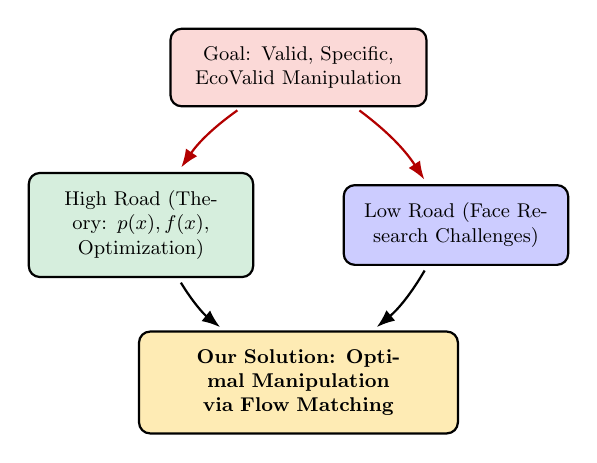
\begin{tikzpicture}[scale=0.8, transform shape, font=\scriptsize]
            \node[conceptbox, fill=myred!20, text width=3.5cm] (problem) at (0,3) {Goal: Valid, Specific, EcoValid Manipulation};
            \node[conceptbox, fill=mygreen!20, text width=3cm] (highroad) at (-2.5,0.5) {High Road (Theory: $p(x), f(x)$, Optimization)};
            \node[conceptbox, fill=blue!20, text width=3cm] (lowroad) at (2.5,0.5) {Low Road (Face Research Challenges)};
            \node[conceptbox, fill=myyellow!30, text width=4.5cm, minimum height=1.5cm] (solution) at (0,-2) {\textbf{Our Solution: Optimal Manipulation via Flow Matching}};

            \draw[arrow,red!70!black] (problem) to[bend right=10] (highroad);
             \draw[arrow,red!70!black] (problem) to[bend left=10] (lowroad);
            \draw[arrow] (highroad) to[bend right=10] (solution);
            \draw[arrow] (lowroad) to[bend left=10] (solution);
        \end{tikzpicture}
    \end{column}
  \end{columns}
  \vfill
  \centering
  \Large{\textbf{Thank You! Questions?}}
  \normalsize
  \vspace{0.2cm}
  Data \& Code: [OSF Link/QR Code], [GitHub Link/QR Code] \\
  Web App: [Link/QR Code]
\end{frame}

\end{document}  
